% Volume III, Chapter 3 -- addendum: transverse Hopf bifurcations of type-cluster equilibria
% (open problem (a) of Remark V3P3:rem:scope).  Verified by code/v3p3_hopf_search.py.
\section{Transverse Hopf bifurcations on \texorpdfstring{$Y_{168}$}{Y168}}\label{V3P3:sec:hopf}

Theorem~\ref{V3P3:thm:clustergrad} excludes Hopf bifurcations inside the cluster subspace, and
Corollary~\ref{V3P3:cor:Y21real} excludes them on $Y_{21}$. On $Y_{168}$ the blocks $M(\lambda)$ of
Theorem~\ref{V3P3:thm:blocks} can have complex spectrum, and the question left open at the end of
Section~\ref{V3P3:sec:twisted} is whether a stable cluster equilibrium can lose stability through a
complex pair of a transverse block, and what happens then. The answer has three parts: the
structure of such a crossing is forced by the symmetry (Proposition~\ref{V3P3:prop:hopfstruct}); such
crossings exist and are common (Theorem~\ref{V3P3:thm:hopf}); and in every case examined the loss
of stability is hard, ending in a frequency-locked state, not on a small limit cycle
(Remark~\ref{V3P3:rem:hopfdyn}). Throughout, $K_1=1$, $\omega_j=\omega$, and the numbers come from
\texttt{code/v3p3\_hopf\_search.py} (numpy, mpmath; seeded; about $25$ minutes; data and figures in
\texttt{data/}).

\begin{proposition}[Structure of a transverse crossing]\label{V3P3:prop:hopfstruct}
Let $\psi$ be a cluster equilibrium, $\lambda\ne0$ an eigenvalue of $A_1$, and $M(\lambda)$ as in
Theorem~\ref{V3P3:thm:blocks}.
\begin{enumerate}
\item[(i)] $M(\omega\lambda)=DM(\lambda)D^{-1}$ with $D=\operatorname{diag}(1,\bar\omega,\omega)$, and
$M(\bar\lambda)=\overline{M(\lambda)}$. So the spectrum of $M(\lambda)$ depends only on the orbit
$[\lambda]$, and if $\lambda^{3}\in\R$ then $M(\lambda)$ is similar to a real matrix.
\item[(ii)] Every eigenvalue $\mu$ of $M(\lambda)$ is an eigenvalue of the Jacobian $J$ with
multiplicity at least $\dim E_\lambda$, and $\bar\mu$ is one of $M(\bar\lambda)$. A crossing of the
imaginary axis at $\mu=i\Omega_H$, $\Omega_H\ne0$, through a transverse block is therefore a Hopf point
at which $i\Omega_H$ and $-i\Omega_H$ each have multiplicity at least $\dim E_\lambda$; the conjugate
comes from $M(\bar\lambda)$ if $[\bar\lambda]\ne[\lambda]$, and from $M(\lambda)$ itself otherwise.
\item[(iii)] On $Y_{168}$ the nonzero eigenvalues of $A_1$ are $7$, the $21$ eigenvalues with
$\lambda^{3}=-1$ (the orbit of $e^{i\pi/3}$, which contains $-1$; $\dim E_\lambda=7$), and the $126$
eigenvalues with $\lambda^{3}=4(5\pm\sqrt{-7})$, i.e.\ $\lambda=2\sqrt2\,e^{\pm i\varphi}\omega^{k}$
with $\varphi=0.162232$ ($\dim E_\lambda=21$ for each sign); $0$ has multiplicity $18$. Hence a
transverse Hopf point through the blocks $2\sqrt2\,e^{\pm i\varphi}$ has $21$ eigenvalues at
$+i\Omega_H$ and $21$ at $-i\Omega_H$, and one through the block of $e^{i\pi/3}$ has a conjugate
pair of multiplicity $7$ each inside the real block $M(-1)$.
\end{enumerate}
\end{proposition}

\begin{proof}
(i) With $d_t=\omega^{-t}$, conjugation by $\operatorname{diag}(d_t)$ multiplies the entry $(t,t+1)$ by
$d_t/d_{t+1}=\omega$ and the entry $(t,t-1)$ by $\bar\omega$, also across the wrap-around $2\to0$,
$0\to2$, since $\omega^{3}=1$. This turns $\alpha_t\lambda$ into $\alpha_t\omega\lambda$ and
$\gamma_t\bar\lambda$ into $\gamma_t\overline{\omega\lambda}$. The coefficients
$\alpha_t,\gamma_t,\sigma_t$ are real, which gives $M(\bar\lambda)=\overline{M(\lambda)}$. If
$\lambda^{3}\in\R$, then $\bar\lambda=\omega^{k}\lambda$ for some $k$, so $M(\lambda)$ is similar to its
complex conjugate; on the orbit of $e^{i\pi/3}$ it is similar to $M(-1)$, which is real. (ii) $J$
acts on $W_{[\lambda]}$ as $M(\lambda)\otimes I_{\dim E_\lambda}$ (Theorem~\ref{V3P3:thm:blocks}), and
$J$ is real. (iii) The spectrum of $A_1$ is computed from the $56$ character blocks of the deck group
$(\Z/2)^{3}\times\Z/7$ (line (A)); the identities $\lambda^{3}=-1$ and $\lambda^{3}=20\pm4\sqrt{-7}$ hold to
$3\cdot10^{-13}$, and the field $\Q(\sqrt{-7})$ is the one met in Chapter~\ref{chap:V3P4},
Remark~\ref{V3P4:rem:blocks}.
\end{proof}

So on $Y_{168}$ no transverse Hopf point is simple, and the classical Hopf theorem, together with
its first Lyapunov coefficient, does not apply. The symmetry group of the problem (the deck
group extended by the lifted automorphisms of $X_3$) acts on the $42$-dimensional real centre
space, and the equivariant Hopf theorem \cite{GSS88} gives a branch of periodic solutions for each
$\C$-axial isotropy subgroup; their direction and stability are decided by the equivariant cubic
normal form, which we have not computed. The numerics below test the dynamics directly.

\begin{theorem}[Transverse Hopf points exist on $Y_{168}$; numerical]\label{V3P3:thm:hopf}
\begin{enumerate}
\item[(a)] Let $K_1=1$, $\alpha=0.55$ and $\Phi=-1.40$. The cluster equilibrium with
$d_0=-1.7681332468697411$, $d_1=2.5493466590522488$ undergoes a transverse Hopf bifurcation in the
block $\lambda=2\sqrt2\,e^{-i\varphi}$ at
\begin{gather*}
K_2^{*}=-0.54407328841619305538826,\qquad \Omega_H=0.0074143951488903915028,\\
\frac{d\operatorname{Re}\mu}{dK_2}\Big|_{K_2^{*}}=5.0116061224789490 .
\end{gather*}
At $K_2^{*}$ the full $168\times168$ Jacobian has exactly $21$ eigenvalues at $i\Omega_H$, $21$ at
$-i\Omega_H$, the rotation eigenvalue $0$, and all others in $\operatorname{Re}\le-0.0180$; the
equilibrium rotates at $\Omega-\omega=-0.0973938$. Along the branch the rest of the spectrum stays
in $\operatorname{Re}<0$ on $[K_2^{*}-0.4,K_2^{*}]$, and the critical pair crosses once, from left to
right. The next crossing is that of a real eigenvalue of the block of $e^{i\pi/3}$, at
$\delta_{\mathrm{next}}=K_2-K_2^{*}=0.0035$; for $0<K_2-K_2^{*}<0.0035$ exactly the $42$ Hopf modes are
unstable.
\item[(b)] Over $150$ random slices $(\alpha,\Phi)$ with $K_2\in[-3,3]$, the $274$ losses of stability of
stable cluster equilibria (rotated copies counted once) are: $191$ real crossings inside the
cluster subspace, $52$ transverse Hopf points, $23$ real crossings of a rate $-\sigma_t$, and $8$ real
crossings in a transverse block. All $52$ Hopf points lie in the blocks $2\sqrt2\,e^{\pm i\varphi}$,
none in the block of $e^{i\pi/3}$, at $K_2\in[-2.74,0.61]$.
\item[(c)] At $\alpha=0.55$, on $72$ values of $\Phi$, there are $26$ Hopf points, on two arcs with
$1.0\lesssim|\Phi|\lesssim2.1$ and $K_2^{*}\in[-2.4,-0.4]$; there $\Omega_H\in[0.0068,0.0074]$, and the
crossing speed $d\operatorname{Re}\mu/dK_2$ is positive at every point.
\end{enumerate}
\end{theorem}

\begin{proof}[Method]
(a) The four real equations ``reduced cluster field $=0$'' and $\det(M(\lambda)-i\omega I)=0$ in the
unknowns $(d_0,d_1,K_2,\omega)$ are solved by Newton's method at $40$ digits, with $\lambda$ computed to
$40$ digits from a character block of $A_1$; the residual is $3\cdot10^{-41}$, and the slope is a
central difference with step $10^{-15}$. This is a high-precision numerical solution of an
analytic system with nonsingular Jacobian, not an interval certificate. The count of eigenvalues
on the axis uses the numerical Jacobian of the $168$ oscillators. (b), (c) Equilibria are found by
vectorized Newton from $36$ seeds at each of $601$ values of $K_2$; each stable one is continued one
step and its leading eigenvalue classified; Hopf points are refined by bisection.
\end{proof}

\begin{figure}[t]
\centering
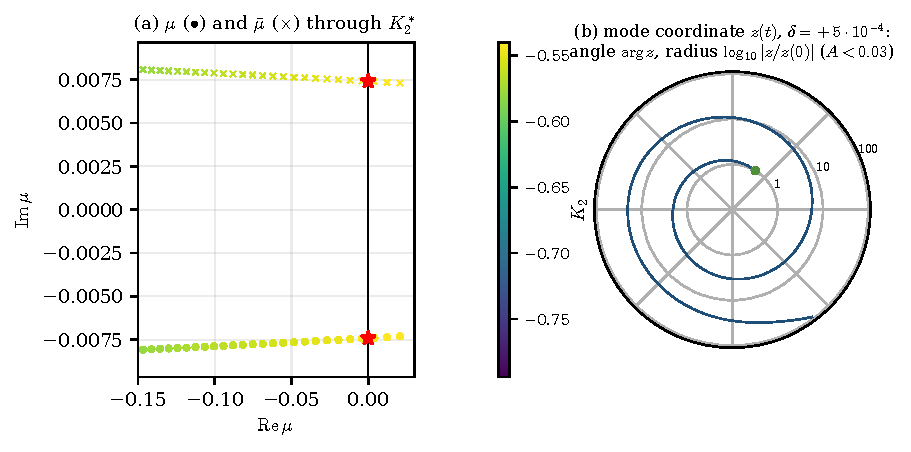
\includegraphics[width=\textwidth]{figures/fig_hopf_orbit.pdf}
\caption{The transverse Hopf point of Theorem~\ref{V3P3:thm:hopf}(a) on $Y_{168}$,
$(K_1,\alpha,\Phi)=(1,0.55,-1.40)$. (a) Along the branch of cluster equilibria, the leading eigenvalue
$\mu$ of the block $M(\lambda)$, $\lambda=2\sqrt2\,e^{-i\varphi}$ (dots), and its conjugate partner
$\bar\mu$ in $M(\bar\lambda)$ (crosses), coloured by $K_2\in[K_2^{*}-0.25,K_2^{*}+0.004]$; they cross the
imaginary axis at $\pm i\Omega_H$, $\Omega_H=0.0074144$ (stars), with speed
$d\operatorname{Re}\mu/dK_2=5.0116$, each with multiplicity $21$. (b) The full $168$-oscillator
network at $K_2=K_2^{*}+5\cdot10^{-4}$, started at amplitude $10^{-4}$ in the $42$-dimensional critical
space: the critical-mode coordinate $z(t)$ in log-polar form (angle $\arg z$, radius
$\log_{10}|z/z(0)|$), shown while the rms deviation $A<0.03$. It turns at the rate $\Omega_H$ and grows at
the linear rate $\operatorname{Re}\mu$ at first, then faster (Remark~\ref{V3P3:rem:hopfdyn}(2)), and
leaves the neighbourhood without settling on a cycle; the trajectory ends in a frequency-locked state.
Drawn by \texttt{code/make\_figures.py}.}
\label{V3P3:fig:hopf}
\end{figure}

\begin{remark}[Numerical: what happens beyond the crossing]\label{V3P3:rem:hopfdyn}
Full-network simulations (RK4, $dt=0.25$) at the point of Theorem~\ref{V3P3:thm:hopf}(a), with
$\delta=K_2-K_2^{*}$:
\begin{enumerate}
\item[(1)] \emph{Linear regime.} For $\delta=+0.0005$ the linearization gives
$\mu=0.00252+0.00740i$. Started at amplitude $10^{-4}$ in the centre space, the rms deviation $A$
grows at rate $0.00255$ and the critical-mode coordinate turns at rate $0.00743$ while
$A\in[2\cdot10^{-4},10^{-3}]$: the instability is the predicted oscillatory one
(Figure~\ref{V3P3:fig:hopf}).
\item[(2)] \emph{No saturation.} The growth then accelerates, to rates $0.0103$ for
$A\in[3\cdot10^{-3},10^{-2}]$ and $0.087$ for $A\in[10^{-2},3\cdot10^{-2}]$: the nonlinearity is
destabilizing, and there is no small-amplitude cycle to land on. The trajectory ends at a state that
is frequency-locked (spread of $\dot\theta_j$ below $2\cdot10^{-13}$) and stationary in the rotating
frame (shape change $4\cdot10^{-16}$), with $A=0.442$ and $r=(0.9994,0.9965,0.8155)$: a relative
equilibrium off the cluster subspace, in which one class is partly desynchronized.
\item[(3)] \emph{All initial directions.} For $\delta=+0.001$ and $+0.002$ (exactly the $42$ Hopf
modes are unstable there), three generic perturbations in the centre space and three pure
character modes (each of the $42$ unstable characters of the deck group spans an invariant
$3$-dimensional subspace) all end in frequency-locked stationary states, with $A$ between $0.40$ and
$0.52$.
\item[(4)] \emph{Below threshold.} The equilibrium is linearly stable, but a perturbation of size
$\varepsilon$ in a fixed generic centre direction escapes to a locked state once
$\varepsilon>\varepsilon_c$, with $\varepsilon_c=0.0053$, $0.0184$, $0.0537$ at $\delta=-0.002$,
$-0.008$, $-0.032$. So $\varepsilon_c\to0$ as $\delta\to0^{-}$, as for a subcritical bifurcation; the
fitted exponent is $0.83$, not the $\frac12$ of a generic cubic normal form, so we do not claim a
normal-form classification.
\item[(5)] \emph{A nearby steady-state crossing.} At every Hopf point examined, a real eigenvalue of
the block of $e^{i\pi/3}$ crosses zero shortly after the Hopf pair: $\delta_{\mathrm{next}}=0.0035$ at
the point of Theorem~\ref{V3P3:thm:hopf}(a), and $0.0005$, $0.0020$, $0.0020$ at three representative
points of (b). This is structural rather than accidental: all blocks share the diagonal $-\sigma_t$, so
when one block reaches the axis the others are close. The transverse Hopf points of $Y_{168}$ thus
sit near a Hopf/steady-state interaction of codimension two.
\item[(6)] \emph{Survey.} At those three representative points, each run at
$\delta=\delta_{\mathrm{next}}/5$ (so that exactly the $42$ Hopf modes are unstable) from a perturbation
of size $10^{-3}$ in the centre space, the outcome is a frequency-locked stationary state in all three
cases ($A=0.27$, $0.22$, $0.32$, each with one class partly desynchronized). An earlier survey of
$12$ Hopf points at $\operatorname{Re}\mu=+0.01$ gave the same outcome in all $12$ cases, with $A$ from
$0.30$ to $1.46$ (at the largest, $r=(0.45,0.45,0.22)$) and $\Omega_H\in[0.0027,0.0076]$.
\item[(7)] \emph{Order parameters.} The critical modes lie in $W_{[\lambda]}\oplus W_{[\bar\lambda]}$,
which is orthogonal to the class indicators (they span $W_{[\kappa]}$, and $A_1$ is normal). So the
class means of the deviation vanish, and $1-r_t=\frac12\operatorname{Var}_{V_t}(\theta)+O(A^{3})$:
the oscillation is visible in $r_0,r_1,r_2$ only at second order, and the time series of the
$r_t$ show the growth (with $1-r_t\propto A^{2}$) and the final jump, not the rotation. The rotation
is seen in the critical-mode coordinate (figure \texttt{v3p3\_hopf\_dynamics.png}).
\end{enumerate}
So transverse Hopf bifurcations exist and account for about a fifth of the losses of stability of
stable cluster states on $Y_{168}$, but no stable limit cycle, chiral or otherwise, was found near
any of them: the loss of stability is hard, and the network freezes into a locked state of the kind
seen in Remark~\ref{V3P3:rem:numerics}(2). This happens even where only the Hopf modes are linearly
unstable, but the nearby steady-state crossing of (5) means that the relevant normal form is that of a
Hopf/steady-state interaction on a $42+7$-dimensional centre space, not of an isolated Hopf point.
Whether some isotropy branch of the equivariant bifurcation is supercritical is open.
\end{remark}

\begin{remark}[Corrections to the proposed programme]\label{V3P3:rem:hopfcorrections}
(1) The crossing is not a simple Hopf bifurcation: on $Y_{168}$ the pair $\pm i\Omega_H$ has
multiplicity $21$ each, forced by the deck-group symmetry (Proposition~\ref{V3P3:prop:hopfstruct}), so
``supercritical'' in the sense of a single first Lyapunov coefficient is not defined. (2) The
bifurcation point $(K_1^{*},K_2^{*},\alpha^{*},\Phi^{*})$ is a curve family, not a point: for fixed
$(\alpha,\Phi)$ there is a value $K_2^{*}$, and Theorem~\ref{V3P3:thm:hopf} gives one to $23$ digits
and the locus at $\alpha=0.55$. (3) Beyond the crossing ($\operatorname{Re}\mu>0$) the simulations do not
produce a stable chiral limit cycle; they produce frequency-locked relative equilibria off the cluster
subspace. (4) The class order parameters $r_t(t)$ see the oscillation only at second order and are
not a good detector of it. (5) The Hopf points are not isolated codimension-one events: a real
crossing in the block of $e^{i\pi/3}$ follows within $\delta_{\mathrm{next}}=0.0005$--$0.0035$.
\end{remark}
